\chapter{Procedure} \label{Sect:procedure}
\section{Quantum Mechanical Data}\label{Sect:procedureData}
\par First-principles calculations were performed within the framework of AFLOW\cite{} which employs the VASP software for computing energies.\cite{} Projector-augmented-wave (PAW) potentials were used and exchange-correlation functionals parametrized by Perdew, Burke, and Ernzerhof under the generalized gradient approximation (GGA)\cite{}. A dense $k$-mesh scheme was used to perform the numeric integration over the Brillioun zone\cite{}. Optimal choices of the unit cells, by standardization of the reciprocal lattice, were adopted to accelerate the convergence of the calculations.
\par As previously discussed, the process of obtaining this data was computationally expensive, creating a bottleneck in the discovery of novelty alloys. The culmination of this research is to produce a simpler model that can be trained on the given data to reproduce expected configuration energies within a range of reasonable error. Fig. \ref{histEnergy} shows a histogram of all the configuration energies in the data set.

\begin{figure}%[h]
\centering
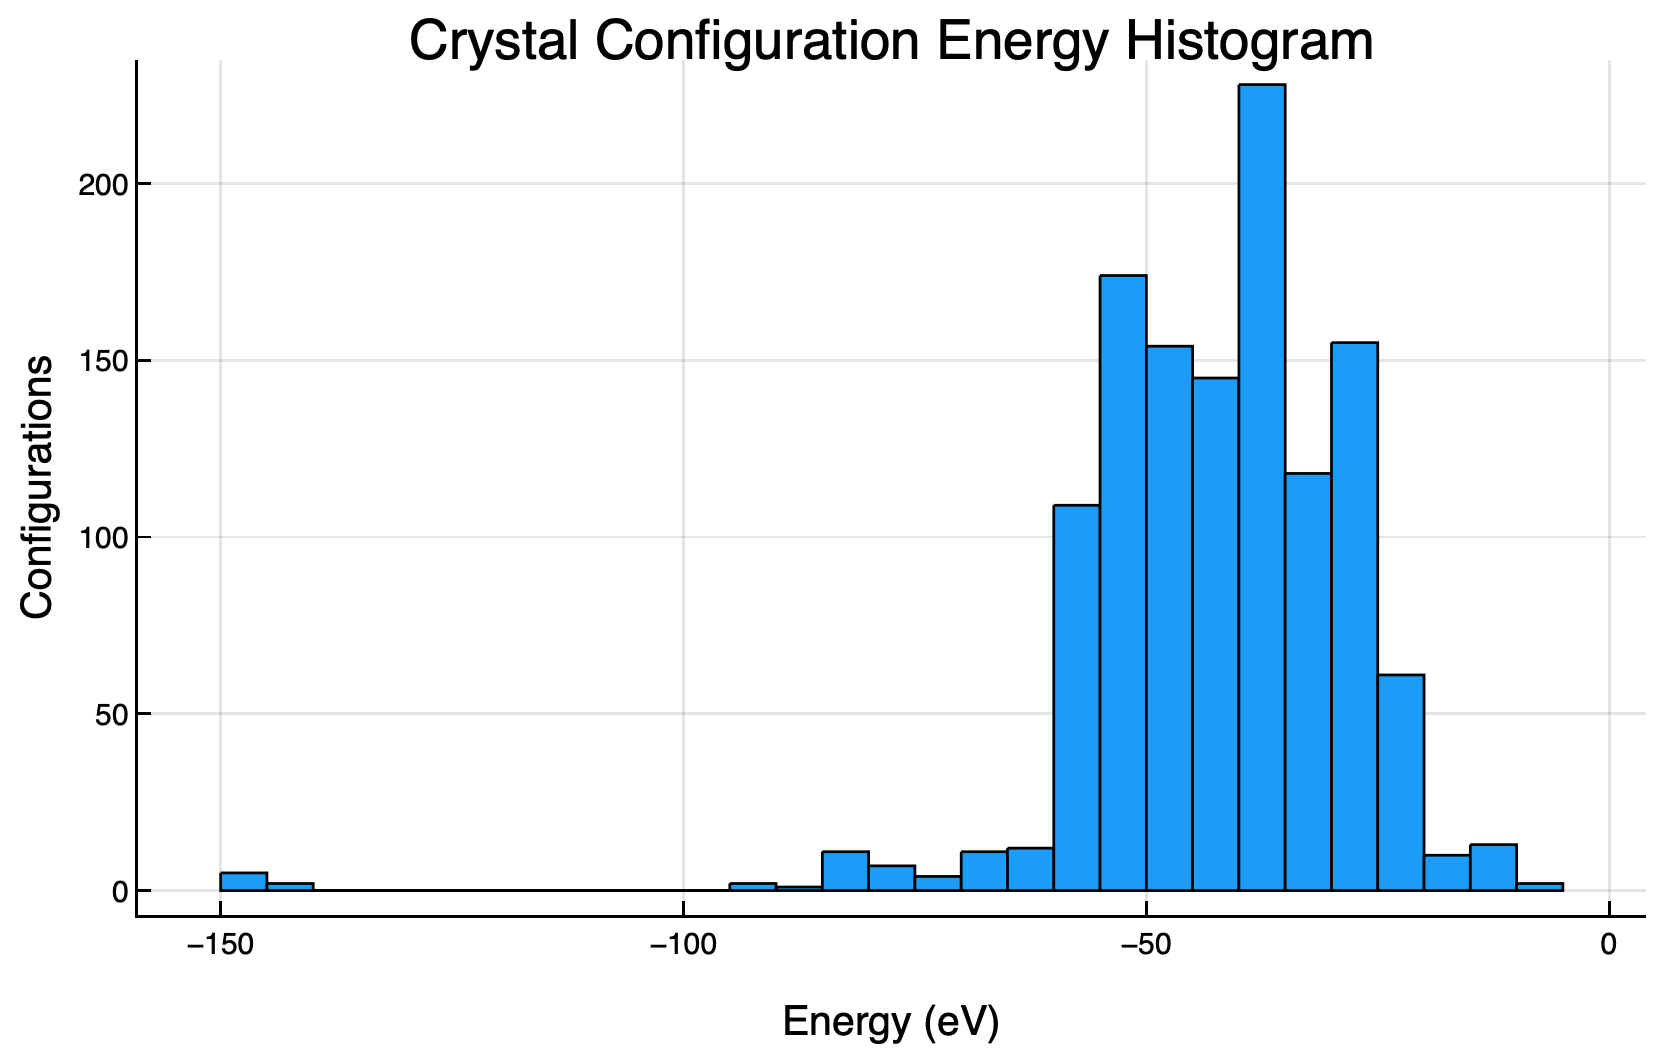
\includegraphics[scale = 0.4]{Figures/UnitCellEnergies}
\caption{A histogram showing all the configuration energies in the original data file. The majority lie within the $-20$eV to $-60$eV range, with a few outliers around $-150$eV.
\label{histEnergy}} 
\end{figure}

\par Each configuration in the data represents a unique primitive unit cell. A unit cell is the building block of any crystal structure. Each unit cell is an identical copy of every other, with the same shape, size, and contents. A \textit{primitive} unit cell is the smallest possible unit cell which contains only one of each uniquely positioned atoms in the crystal\cite{solidStateBook}. An example of a primitive unit cell configuration can be seen in fig. \ref{primitiveUnitCells}.

\begin{figure}
  \centering
  \begin{subfigure}{0.53\textwidth}
    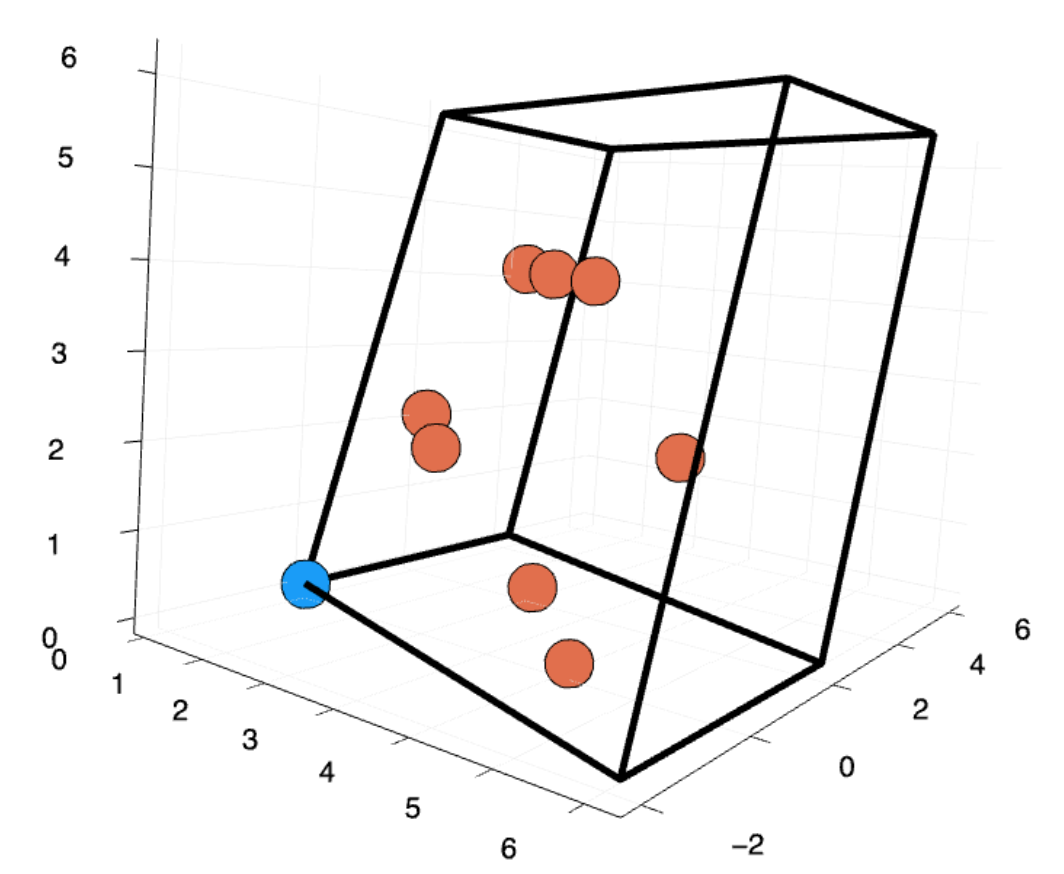
\includegraphics[width=\linewidth]{Figures/primitiveCell1}
    %\caption{First subfigure} 
    \label{primitiveFirst}
  \end{subfigure}%
  \hspace*{\fill}   % maximize separation between the subfigures
  \begin{subfigure}{0.49\textwidth}
    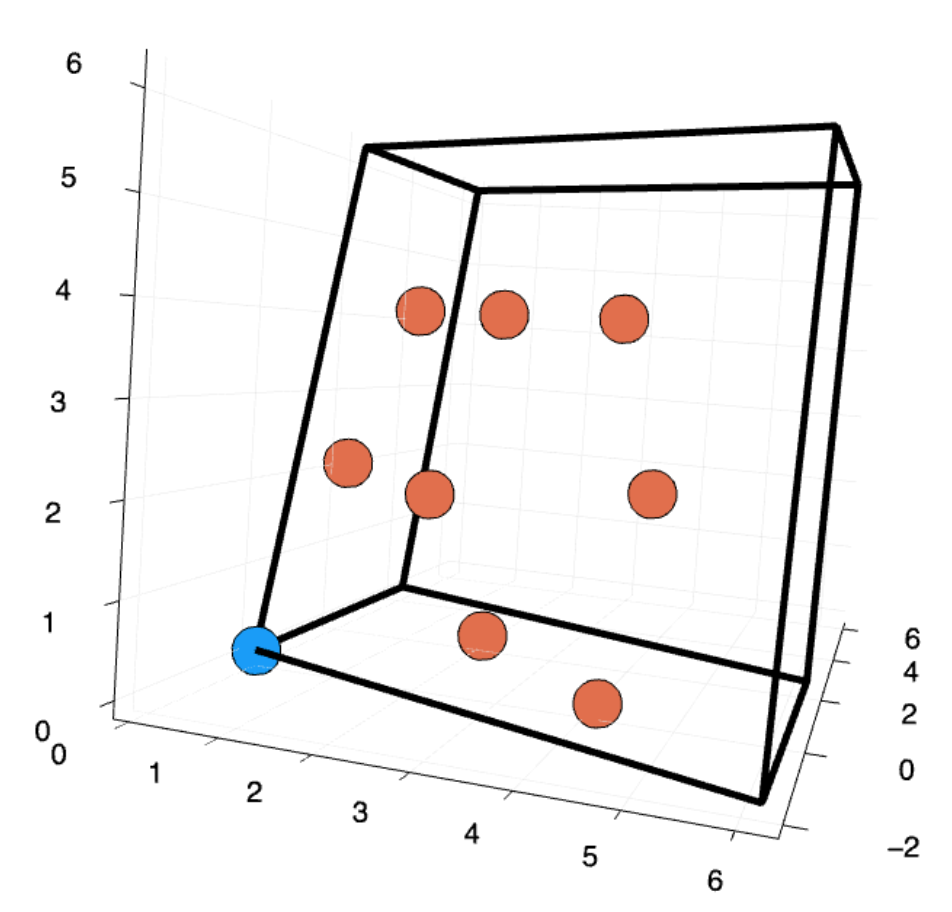
\includegraphics[width=\linewidth]{Figures/primitiveCell2}
    %\caption{Second subfigure} 
    \label{primitiveSecond}
  \end{subfigure}%
\caption{The primitive unit cell for configuration 65 from two different perspectives. The blue point is the single Ag atom while each red point shows each Pt atom in said configuration.} \label{primitiveUnitCells}
\end{figure}

\par To use the data in the \textit{.txt} file, it needs to be parsed into vectors that can be easily manipulated. An example of the data being parsed can be seen in fig. \ref{system2data}. The number on the second line is the lattice parameter, followed by three lattice vectors in $(i,j,k)$ coordinates. The line following contains two numbers, the first is the number of silver (Ag) atoms in the unit cell and the second is the number of platinum (Pt) atoms. In direct coordinates (in terms of the lattice vectors) the positions of each silver and platinum atom are then given. The last line in this system tells the total potential energy of the unit cell configuration. 

\begin{figure}%[h]
\centering
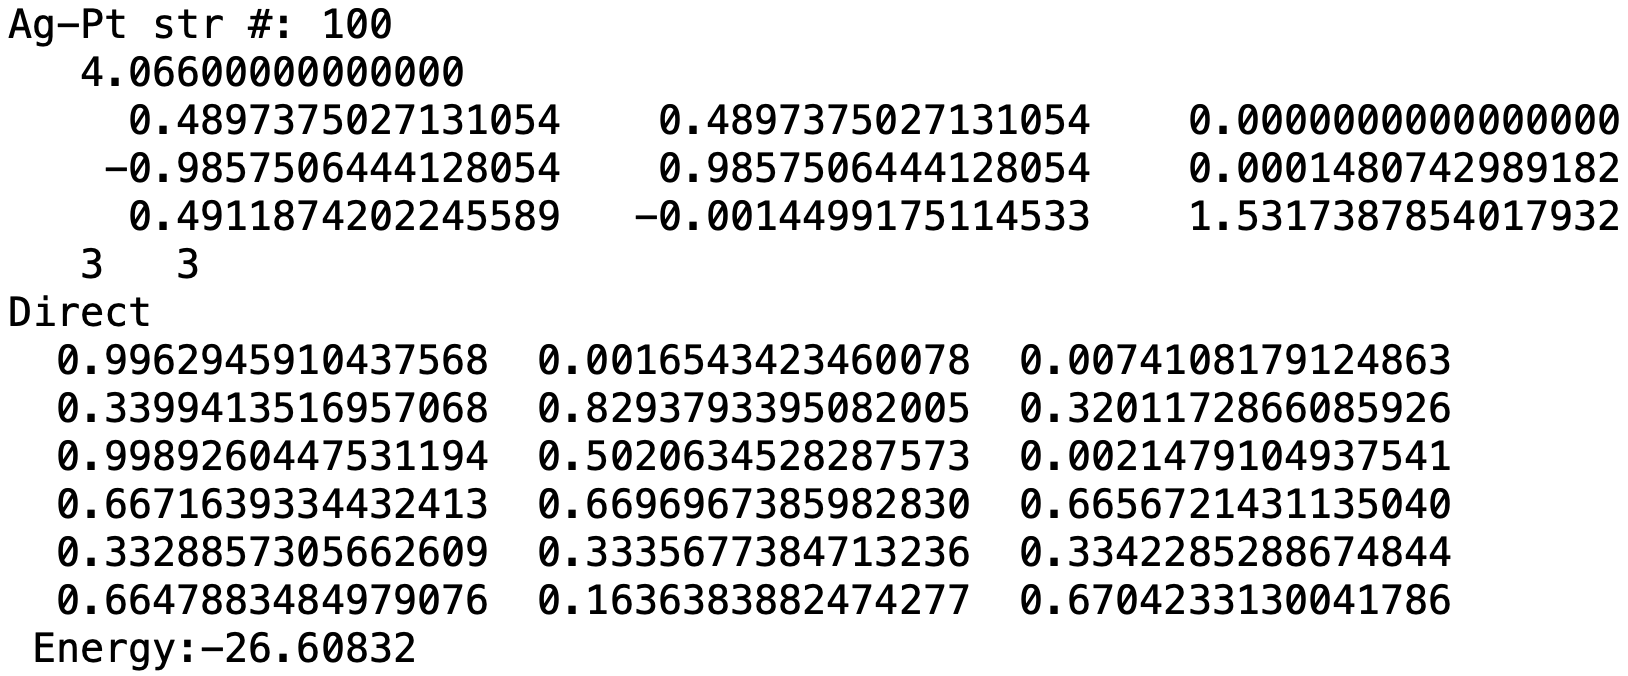
\includegraphics[scale = 0.4]{Figures/system2}
\caption{An example of the data given in AgPtdata.txt that needs to be used to build the model.
\label{system2data}} 
\end{figure}

\section{Model Construction}\label{Sect:procedureConstruction}
\par With the file parsed and the important data retrieved, the process of building a model can commence. The potential energy of a single particle is due to its interactions with all its surrounding particles, thus to account for each interaction with nearby particles the unit cell must be propagated outwards in all three dimensions. All atomic pairs can be enumerated by adding multiples of the lattice vectors. Then the relative position of each affecting particle can be determined and the vector separating the particle pair can be calculated. These separation vectors are the information that will be passed into the basis function to construct the model. 
\par Because the affect two particles have on each other drops off as a function of distance (similar to the Lennard-Jones potential), the unit cell does not need to be propogated infinitely in each direction, only out to a radius of reasonable influence, creating an imaginary sphere beyond which all interactions are negligible. It should be clear that the choice of this radius will make a significant impact on the quality of the model. It should also be noted that one arbitrarily chosen radius cannot be applied effectively to each unique system. A simple solution is to make the radius of this sphere of influence equal to the magnitude of the largest lattice vector multiplied by a constant. The effect of this constant on the model's precision can be tested later, but for now will be chosen to be 1.2.
\par The simplification of reality due to this ``sphere of influence" gives a clear upper bound to our unit cell propagation. It is expected that the unit cell will be propagated out further than the radius in each direction, thus encapsulating said sphere. An example of this iterated unit cell can be seen in fig. \ref{iteratedUnitCells}. 

\begin{figure}
  \centering
  \begin{subfigure}{0.53\textwidth}
    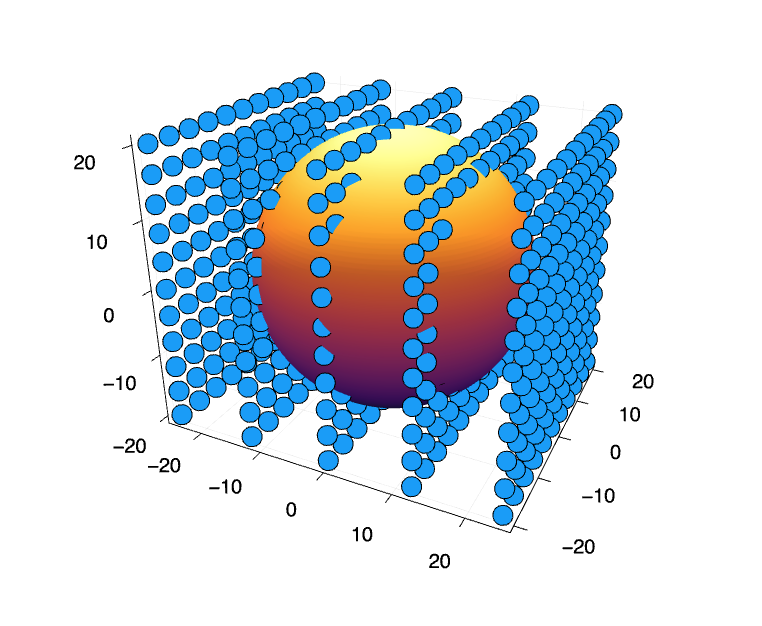
\includegraphics[width=\linewidth]{Figures/iteratedUnitCell}
    %\caption{First subfigure} 
    \label{iteratedUnitCellFirst}
  \end{subfigure}%
  %\\
  \hspace*{\fill}   % maximize separation between the subfigures
  \begin{subfigure}{0.5\textwidth}
    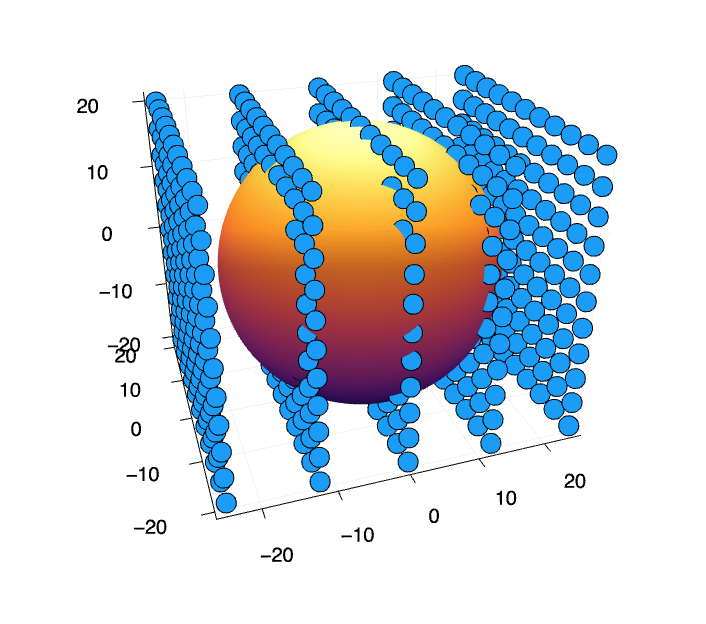
\includegraphics[width=\linewidth]{Figures/iteratedUnitCell2}
    %\caption{Second subfigure} 
    \label{iteratedUnitCellSecond}
  \end{subfigure}
\caption{The sphere of influence for one silver atom is completely encapsulated by the unit cell's iterations from two different perspectives. Only one particle from each unit cell is shown.} \label{iteratedUnitCells}
\end{figure}

Each unit cell in fig. \ref{iteratedUnitCells} can now be populated with all the contained atoms. Every atom inside the sphere can then be extracted. When these atoms are stored into a new vector, they can be plotted as in fig. \ref{plotAgAtomSphere}. When this process is repeated for every system in the DFT data, the result is a vector containing these ``important positions" for each unique silver and platinum atom in each unit cell. The separation vector norms can be quickly calculated and stored.

\begin{figure}%[h]
\centering
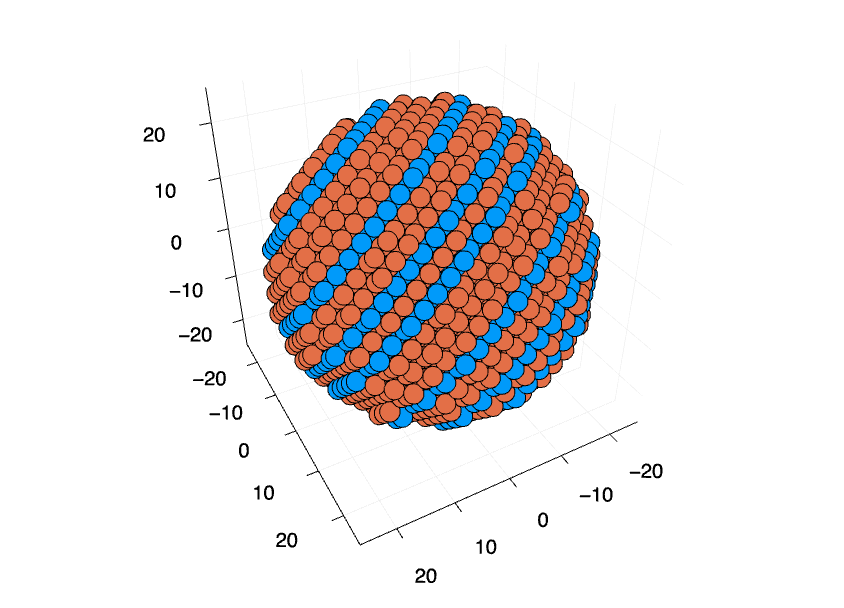
\includegraphics[scale = 0.65]{Figures/plotAgAtomSphere(3,1)}
\caption{Every silver and platinum atom inside the sphere of interest. According to the model, these are the only atoms interacting with the central atom in question. This data is taken from the first silver atom in the third configuration. 
\label{plotAgAtomSphere}} 
\end{figure}

With all the pertinent information from the data organized into vectors, construction of the $\mathbf{A}$ matrix can begin. As in the Lennard-Jones example, each row represents a crystal structure and each column corresponds to a unique basis function. And as explained in Section \ref{Sect:diatomic}, a single basis function will result in three columns of $\mathbf{A}$ due to each type of interaction. The method of populating $\mathbf{A}$ will be the same as was done earlier in eq. \ref{eq:fillBessel}. With 300 basis functions, the first 300 columns of $\mathbf{A}$ will be calculated using the separation vector norms from Ag-Ag interactions. The following 300 columns from Pt-Pt interactions and the final 300 from Ag-Pt.
\par The size of the training set is limited to 1224, the number of systems given in the data set. Whatever systems are not included in the training set will comprise the holdout set, used for testing the model's accuracy.
%\par The basis functions will again be chosen to be bessel functions of the second kind. This is because of the similarity in potential energy between two atoms as a function of distance and the shape of the graph of said bessel functions. 
\par Once the model is fully constructed, tests can be run to determine the effect of radius, size of training set, and number of basis functions on the precision and accuracy of the model. An increase of these three variables will make significant impacts on the program runtime. As the radius is increased, the unit cell must be propagated out further to encapsulate the sphere of influence and more atom interactions will be considered. For every basis function added, there will be three columns added to the $\mathbf{A}$ matrix, drawing out its construction times. 
\par Generally, as the number of basis functions is increased and the radius of influence extended, the model's predictions will become increasingly reliable. On the other hand, as those factors increase accuracy and precision, they also increase the computational costs. It would be ideal to find a manageable trade off between the program's runtime and reliability. To investigate the quality of the model as a function of cutoff radius, size of training set, and number of basis functions, a sweep can be conducted over a range of values for each and the details of the fit for each combination can be recorded. Rather than run this script on an ordinary desktop computer, it was completed on Mary Lou, BYU's supercomputer. 
